\textbf{Цель работы:} измерение магнитной восприимчивости диа- и парамагнитного образцов.

\textbf{В работе используются:} электромагнит, аналитические весы, милливеберметр, регулируемый источник постоянного тока, образцы.
                    
\section{Теоретическое введение}

Магнитная восприимчивость тел может быть определена по измерению сил, действующих на тела в магнитном поле. В одном из способов (метод Гюи) используется
тонкий и длинный стержень, один из концов которого помещают в зазор электромагнита (обычно в область однородного поля), а другой конец -- вне зазора, где величиной магнитного поля можно пренебречь. Закон изменения поля -- от максимального до нулевого -- в этом случае несуществен.

В этом случае сила, действующая на стержень, имеет вид:

\begin{equation}
    F_M = \left( \frac{\partial W_M}{\partial x} \right)_I
\end{equation}

Используя выражение для плонтости энергии магнитного поля, легко получить, что

\begin{equation}
    dW_M(\Delta x) \approx \mu \frac{B_0^2}{2 \mu_0} S dx - \frac{B_0^2}{2 \mu_0} S dx = (\mu - 1) \frac{B_0^2}{2 \mu_0} S dx
\end{equation}

Здесь $B_0$ -- идукция магнитного поля электромагнита. Формула выше получена с помощью следующих приближений: магнитная восприимчивость тела мала $\mu \approx 1$, значит можно воспользоваться граничными условиями на магнитную напряжённость.

Таким образом,

\begin{equation}
    F_M = \chi \frac{B_0^2}{2 \mu_0} S
\end{equation}

\section{Экспериментальная установка}

Магнитное поле с максимальной индукцией $\approx 1$ Тл создаётся в зазоре электромагнита, питаемого постоянным током. Диаметр полюсов существенно превосходит ширину зазора, поэтому поле в средней части зазора достаточно однородно. Величина тока, проходящего через обмотки электромагнита, задаётся регулируемым источником постоянного напряжения.

\begin{figure}[h]
    \centering
    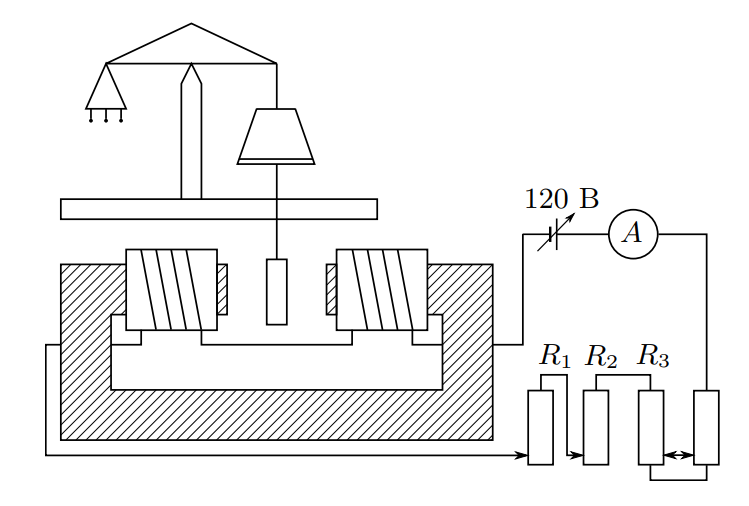
\includegraphics[width = 10 cm]{images/1.png}
    \caption{Схема экспериментальной установки}
    \label{eksp_ust}
\end{figure}

При измерениях образцы поочерёдно подвешиваются к аналитическим весам так, что один конец образца оказывается в зазоре электромагнита, а другой — вне зазора, где индукцией магнитного поля можно пренебречь. При помощи аналитических весов определяется перегрузка $\Delta P = F$ -- сила, действующая на образец со стороны магнитного поля.

Градуировка электромагнита (связь между индукцией магнитного поля $B$ в зазоре электромагнита и силой тока $I$ в его обмотках) производится при помощи милливеберметра.

\section{Ход работы}

\subsection{Калибровка электромагнита}

Снимем зависимость $B(I)$, учитывая, что $SN = 72 \; \text{см}^2$:

\begin{table}[h!]
    \begin{tabular}{|c|c|c|c|c|c|c|c|c|c|c|}
    \hline
    \textbf{$I$, А}   & 0,3   & 0,6   & 0,9   & 1,2   & 1,5   & 1,8   & 2,1   & 2,4   & 2,7   & 3     \\ \hline
    \textbf{Ф, мВб}   & 0,75  & 1,5   & 2,2   & 2,95  & 3,65  & 4,4   & 5     & 5,6   & 6,2   & 6,7   \\ \hline
    \textbf{$B$, мТл} & 104,2 & 208,3 & 305,6 & 409,7 & 506,9 & 611,1 & 694,4 & 777,8 & 861,1 & 930,6 \\ \hline
    \end{tabular}
\end{table}

Построим градуировочную кривую:

\begin{figure}[h!]
    \centering
    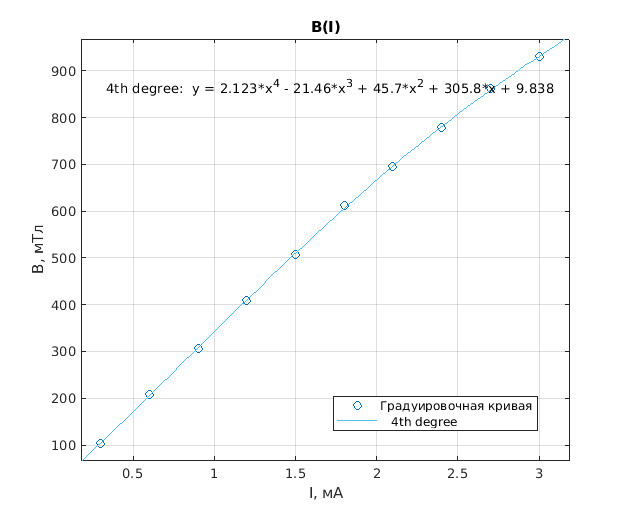
\includegraphics[width = 13 cm]{images/grad.png}
    \caption{Градуировочная кривая}
    \label{grad}
\end{figure}

Кривую удобно аппроксимировать полиномом четвёртой степени, тогда можно находить точки на этой кривой с помощью формулы полинома.

Все дальнейшие данные для замены токов значениями магнитного поля будут браться из градуировочной кривой.

\subsection{Измерение зависимости $F(B^2)$}

\subsubsection{Алюминиевый стержень}

Снимем зависимость $F(I)$, после чего строим таблицу для $F(B^2)$.

\begin{table}[h!]
    \begin{tabular}{|c|c|c|c|c|c|c|}
    \hline
    \textbf{$F$, мН}               & 0,13734 & 0,14715 & 0,18639 & 0,20601 & 0,24525 & 0,26487 \\ \hline
    \textbf{$B^2$, $\text{мТл}^2$} & 256992  & 312508  & 373456  & 426115  & 482253  & 541850  \\ \hline
    \textbf{$F$, мН}               & 0,30411 & 0,33354 & 0,37278 & 0,40221 & 0,43164 &         \\ \hline
    \textbf{$B^2$, $\text{мТл}^2$} & 604938  & 671483  & 741512  & 802516  & 865933  &         \\ \hline
    \end{tabular}
    \caption{Таблица для алюминия}
\end{table}

Построим график зависимости.

\begin{figure}[h]
    \centering
    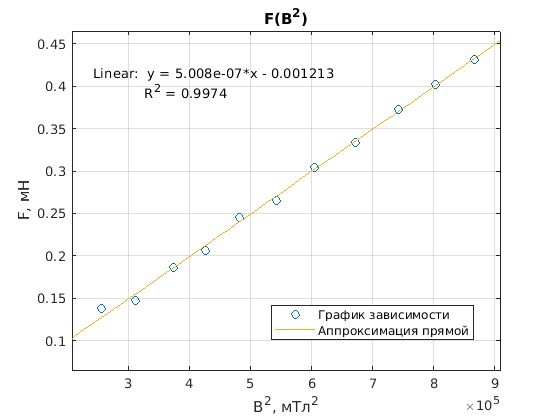
\includegraphics[width = 12 cm]{images/al.png}
    \caption{График для алюминия}
    \label{al}
\end{figure}

Из зависимости имеем $k = (5,01 \pm 0,17) \cdot 10^{-10} \; \frac{\text{Н}}{\text{Тл}^2}$, откуда следует, что $\chi = (1,60 \pm 0,07) \cdot 10^{-11}$. 

\subsubsection{Графитовый стержень №1}

Снимем зависимость $F(I)$, после чего строим таблицу для $F(B^2)$.

\begin{table}[]
    \centering
    \begin{tabular}{|c|l|l|l|l|l|}
    \hline
    \textbf{$F$, мН}               & 0,1079 & 0,3237 & 0,5493 & 0,7651 & 1,0300 \\ \hline
    \textbf{$B^2$, $\text{мТл}^2$} & 10850  & 43407  & 93364  & 167872 & 256992 \\ \hline
    \textbf{$F$, мН}               & 1,2262 & 1,4028 & 1,5410 & 1,8541 & 2,0601 \\ \hline
    \textbf{$B^2$, $\text{мТл}^2$} & 373456 & 482253 & 604938 & 741512 & 865933 \\ \hline
    \end{tabular}
    \caption{Таблица для графита №1}
\end{table}

Построим график зависимости.

\begin{figure}[h]
    \centering
    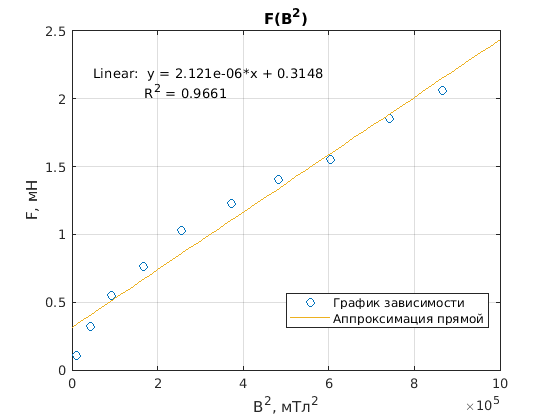
\includegraphics[width = 12 cm]{images/gr.png}
    \caption{График для графита №1}
    \label{gr1}
\end{figure}

Из зависимости имеем $k = (2,12 \pm 0,22) \cdot 10^{-9} \; \frac{\text{Н}}{\text{Тл}^2}$, откуда следует, что $\chi = (6,65 \pm 0,71) \cdot 10^{-11}$. 

\subsubsection{Графитовый стержень №2}

Снимем зависимость $F(I)$, после чего строим таблицу для $F(B^2)$.

\begin{table}[]
    \centering
    \begin{tabular}{|c|l|l|l|l|l|}
    \hline
    \textbf{$F$, мН}               & 0,1275 & 0,3728 & 0,6377 & 0,9221 & 1,1968 \\ \hline
    \textbf{$B^2$, $\text{мТл}^2$} & 10850  & 43407  & 93364  & 167872 & 256992 \\ \hline
    \textbf{$F$, мН}               & 1,5206 & 1,8247 & 2,1386 & 2,4231 & 2,6781 \\ \hline
    \textbf{$B^2$, $\text{мТл}^2$} & 373456 & 482253 & 604938 & 741512 & 865933 \\ \hline
    \end{tabular}
    \caption{Таблица для графита №2}
\end{table}

Построим график зависимости.

\begin{figure}[h]
    \centering
    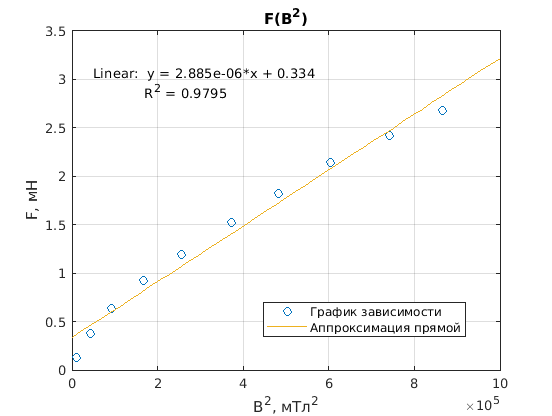
\includegraphics[width = 12 cm]{images/gr2.png}
    \caption{График для графита №2}
    \label{gr1}
\end{figure}

Из зависимости имеем $k = (2,89 \pm 0,24) \cdot 10^{-9} \; \frac{\text{Н}}{\text{Тл}^2}$, откуда следует, что $\chi = (9,06 \pm 0,72) \cdot 10^{-11}$.

\section{Заключение}

Таким образом изначальная модель зависимости $F(B)$ оказалась верна, а при рабочих значения индукции магнитного поля значения магнитной воприимчивости оказались практически постоянными (но видны отклонения при возрастании магнитной индукции электромагнита). Были получены следующие значения магнитной восприимчивости для разных материалов:

Для алюминия $\chi = (1,60 \pm 0,07) \cdot 10^{-11}$.

Для графита (первый стержень) $\chi = (6,65 \pm 0,71) \cdot 10^{-11}$. 

Для графита (второй стержень) $\chi = (9,06 \pm 0,72) \cdot 10^{-11}$.

























